% ----------------------------------------------------------------------------
%
%                           Hydrology
%                                  Cookbook
%
% ----------------------------------------------------------------------------
%
%

\documentclass[landscape]{article}
\fontsize{6}{10}\selectfont
\usepackage[light, frenchstyle,narrowiints,partialup]{kpfonts}
\usepackage{array}
\usepackage{amsmath,amssymb}
\usepackage{booktabs}
\usepackage{caption}
\usepackage[nodayofweek]{datetime}
\usepackage{environ}
\usepackage{float}
\usepackage{enumitem}
\usepackage{fancyhdr}
\usepackage[landscape,margin=13mm,footskip=1pt,includefoot]{geometry}
\usepackage{graphicx}
\usepackage{hyperref}
\usepackage{multicol}
\usepackage{rotating}
\usepackage{threeparttable}
\usepackage{url}
\usepackage{xspace}
\usepackage{mathabx}
\usepackage{footnote}
\usepackage{tablefootnote}
\usepackage{mathtools}
\usepackage[compact]{titlesec}
\usepackage[english]{babel}

\usepackage[backend=biber]{biblatex}
\addbibresource{./literature.bib}
\usepackage{xcolor}

% Document version, MAJOR.MINOR.PATCH. Please change with any modification
% according to semantic versioning practices:
%   - The major version changes when adding a new section or topic, or making a
%     substantial content change.
%   - The minor version changes for non-trivial fixes, corrections, or
%     improvements.
%   - The patch version changes for trivial fixes, such as typos in text or
%     formulas.
\newcommand{\version}{3.0}

% Probability and Statistics LaTeX shortcuts.
\usepackage{amsmath,amssymb}
\usepackage{dsfont}
\usepackage{cancel}
\usepackage{graphicx}
\usepackage{xargs}
\usepackage{xspace}

% =============================================================================
%                                  Formatting
% =============================================================================

% Make a note on the margin.
\newcommand{\marnote}[1]{
  \reversemarginpar
  \marginpar[\raggedleft\footnotesize\textit{\\[3ex]#1}]%
      {\raggedright\footnotesize\textit{\\[3ex]#1}}
  \normalmarginpar
}

\newcommand{\pwiseii}[1]{\ensuremath{\left\{\begin{array}{ll}#1\end{array}}}
\newcommand{\pwiseiii}[1]{\ensuremath{\left\{\begin{array}{ll}#1\end{array}}}
\newcommand{\prn}[1]{\ensuremath{\left(#1\right)}}
\newcommand{\brk}[1]{\ensuremath{\left[#1\right]}}
\newcommand{\brc}[1]{\ensuremath{\left\{#1\right\}}}
\newcommand{\x}[1]{\ensuremath{\cancel{#1}}}

% =============================================================================
%                                 General Math
% =============================================================================

% Special functions and operators
\DeclareMathOperator{\erf}{erf}
\DeclareMathOperator{\logit}{logit}
\DeclareMathOperator{\sign}{sign}
\DeclareMathOperator*{\argmin}{\arg\!\min}

% Definitions
\def\define{:=}
\def\defined{=:}
\def\eqdef{\triangleq}

% Proofs
\def\qed{\ifhmode\unskip\nobreak\fi\hfill \ensuremath{\square}}

% Standard transformation function
\def\transform{\ensuremath{\varphi}\xspace}

% Logic
\newcommand{\comp}[1]{\neg{#1}}
\newcommand{\imp}{\ensuremath{\;\Longrightarrow\;}}
\newcommand{\pmi}{\ensuremath{\;\Longleftarrow\;}}
\newcommand{\nimp}{\ensuremath{\;\not\!\!\Longrightarrow\;}}
\newcommand{\npmi}{\ensuremath{\;\not\!\!\Longleftarrow\;}}
\newcommand{\eqv}{\ensuremath{\;\Longleftrightarrow\;}}

% Numbers.
\def\C{\mathbb{C}}
\def\N{\mathbb{N}}
\def\R{\mathbb{R}}
\def\Z{\mathbb{Z}}

% Matrices
\newcommand{\eyeii}{\ensuremath{\left(\begin{matrix}1 & 0 \\ 0 & 1\end{matrix}\right)}}
\newcommand{\eyeiii}{\ensuremath{\left(\begin{matrix}1 & 0 & 0 \\ 0 & 1 & 0 \\ 0 & 0 & 1\end{matrix}\right)}}

% Limits
\newcommand{\Lim}[2]{\ensuremath{\lim_{#1\to #2}}}
\newcommand{\limx}[1][\infty]{\ensuremath{\lim_{x\to #1}}}
\newcommand{\limn}[1][\infty]{\ensuremath{\lim_{n\to #1}}}

% Sums and products
\newcommand{\Sum}[2][i=1]{\ensuremath{\sum_{#1}^{#2}}}
\newcommand{\sumin}{\ensuremath{\sum_{i=1}^n}}
\newcommand{\sumiN}{\ensuremath{\sum_{i=1}^N}}
\newcommand{\sumim}{\ensuremath{\sum_{i=1}^m}}
\newcommand{\sumjk}{\ensuremath{\sum_{j=1}^k}}
\newcommand{\sumjn}{\ensuremath{\sum_{j=1}^n}}
\newcommand{\sumjm}{\ensuremath{\sum_{j=1}^m}}
\newcommand{\isum}[1][n]{\ensuremath{\sum_{#1}^\infty}}
\newcommand{\dsum}[4][i=1]{\ensuremath{\sum_{#1}^{#2}\sum_{#3}^{#4}}}
\newcommand{\Prod}[2][i=1]{\ensuremath{\prod_{#1}^{#2}}}
\newcommand{\prodin}{\ensuremath{\prod_{i=1}^n}}
\newcommand{\prodjn}{\ensuremath{\prod_{j=1}^n}}

% Derivatives
\newcommand{\der}[2][]{\ensuremath{\frac{d #1}{d #2}}}
\newcommand{\dder}[2][]{\ensuremath{\frac{d^2 #1}{d #2^2}}}
\newcommand{\pder}[2][]{\ensuremath{\frac{\partial #1}{\partial #2}}}
\newcommand{\pdder}[2][]{\ensuremath{\frac{\partial^2 #1}{\partial #2^2}}}
\newcommand{\mpder}[3][]{%
  \ensuremath{\frac{\partial^2 #1}{\partial #2 \partial #3}}}
\newcommand{\at}[2][]{#1|_{#2}}

% Differentials
%\renewcommand{\d}[1]{\,\mathrm{d}#1}
\renewcommand{\d}[1]{\,d#1}
\def\ds{\d{s}}
\def\dt{\d{t}}
\def\dtheta{\d{\theta}}
\def\du{\d{u}}
\def\dx{\d{x}}
\def\dy{\d{y}}
\def\dfx{\d{F_X(x)}}
\def\dfy{\d{F_Y(y)}}
\def\dfhatx{\d{\widehat{F}_n(x)}}

% Transcendentals w/ extended arguments.
\newcommand{\Exp}[1]{\ensuremath{\exp\left\{#1\right\}}}
\newcommand{\Log}[1]{\ensuremath{\log\left\{#1\right\}}}

% =============================================================================
%                          Probability and Statistics
% =============================================================================

% Formatted terminology.
\def\bias{\textsf{bias}\xspace}
\def\se{\textsf{se}\xspace}
\def\pdf{\textsc{pdf}\xspace}
\def\cdf{\textsc{cdf}\xspace}
\def\ise{\textsc{ise}\xspace}
\def\pgf{\textsc{pgf}\xspace}
\def\mgf{\textsc{mgf}\xspace}
\def\mse{\textsc{mse}\xspace}
\def\mspe{\textsc{mspe}\xspace}
\def\mle{\textsc{mle}\xspace}
\def\mom{\textsc{mom}\xspace}
\def\are{\textsc{are}\xspace}
\def\rss{\textsc{rss}\xspace}
\def\ess{\textsc{ess}\xspace}
\def\tss{\textsc{tss}\xspace}

% Naming shortcuts.
\def\ahat{\ensuremath{\widehat{\alpha}}}
\def\atil{\ensuremath{\tilde{\alpha}}}
\def\bhat{\ensuremath{\widehat{\beta}}}
\def\btil{\ensuremath{\tilde{\beta}}}
\def\dhat{\ensuremath{\widehat{\delta}}}
\def\ehat{\ensuremath{\hat{\epsilon}}}
\def\ghat{\ensuremath{\widehat{\gamma}}}
\def\khat{\ensuremath{\widehat{\kappa}}}
\def\lhat{\ensuremath{\widehat{\lambda}}}
\def\ltil{\ensuremath{\tilde{\lambda}}}
\def\mhat{\ensuremath{\widehat{\mu}}}
\def\nhat{\ensuremath{\widehat{\nu}}}
\def\mtil{\ensuremath{\tilde{\mu}}}
\def\psihat{\ensuremath{\widehat{\psi}}}
\def\shat{\ensuremath{\widehat{\sigma}}}
\def\stil{\ensuremath{\tilde{\sigma}}}
\def\that{\ensuremath{\widehat{\theta}}}
\def\ttil{\ensuremath{\widetilde{\theta}}}
\def\rhohat{\widehat{\rho}}
\def\xihat{\widehat{\xi}}

\def\sehat{\ensuremath{\widehat{\se}}}
\def\fhat{\ensuremath{\widehat{f}}}
\def\Fhat{\ensuremath{\widehat{F}}}
\def\fnhat{\ensuremath{\widehat{f}_n}}
\def\Fnhat{\ensuremath{\widehat{F}_n}}
\def\Jhat{\ensuremath{\widehat{J}}}
\def\phat{\ensuremath{\widehat{p}}}
\def\ptil{\ensuremath{\tilde{p}}}
\def\rhat{\widehat{r}}
\def\Rbar{\bar{R}}
\def\Rhat{\widehat{R}}
\def\Qbar{\bar{Q}}
\def\Qhat{\widehat{Q}}
\def\Xhat{\widehat{X}}
\def\xbar{\bar{x}}
\def\Xbar{\bar{X}}
\def\Xsqbar{\overline{X^2}}
\def\xnbar{\overline{x}_n}
\def\Xnbar{\overline{X}_n}
\def\Yhat{\widehat{Y}}
\def\ybar{\overline{y}}
\def\Ybar{\overline{Y}}
\def\Ynbar{\overline{Y}_n}

% Random variables.
\def\rv{\textsc{rv}\xspace}
\def\iid{\ensuremath{\textsc{iid}}\xspace}
\def\dist{\ensuremath{\sim}\xspace}
\def\disteq{\ensuremath{\stackrel{D}{=}}\xspace}
\def\distiid{\ensuremath{\stackrel{iid}{\sim}}\xspace}
\def\ind{\ensuremath{\perp\!\!\!\perp}\xspace}
\def\nind{\ensuremath{\perp\!\!\!\!\big\vert\!\!\!\!\perp}\xspace}
\def\Xon{\ensuremath{X_1,\dots,X_n}\xspace}
\def\xon{\ensuremath{x_1,\dots,x_n}\xspace}
\def\giv{\ensuremath{\,|\,}}
\def\Giv{\ensuremath{\,\big|\,}}
\def\GIV{\ensuremath{\,\Big|\,}}
\newcommand{\indicator}[1]{\mathds{1}_{\left\{#1\right\}}}

% Probability, expectation, and variance.
\def\prob{\mathbb{P}}
\renewcommand{\Pr}[2][]{\ensuremath{\prob_{#1}\left[#2\right]}\xspace}
\newcommand{\E}[2][]{\ensuremath{\mathbb{E}_{#1}\left[#2\right]}}
\newcommand{\V}[2][]{\ensuremath{\mathbb{V}_{#1}\left[#2\right]}}
\newcommand{\cov}[2][]{\ensuremath{\mathrm{Cov}_{#1}\left[#2\right]}}
\newcommand{\corr}[2][]{\ensuremath{\rho_{#1}\left[#2\right]}}
\def\sd{\ensuremath{\textsf{sd}}\xspace}
\def\samplemean{\ensuremath{\bar{X}_n}\xspace}
\def\samplevar{\ensuremath{S^2}\xspace}
\def\za{\ensuremath{z_{\alpha}}}
\def\zat{\ensuremath{z_{\alpha/2}}}

% Inference
\def\Ll{\ensuremath{\mathcal{L}}\xspace}
\def\Lln{\ensuremath{\Ll_n}\xspace}
\def\ll{\ensuremath{\ell}}
\def\lln{\ensuremath{\ll_n}}

% Hypothesis testing
\newcommand{\hyp}[2]{
\ensuremath{H_0:#1 \ifhmode\quad\text{versus}\quad\fi\text{ vs. } H_1:#2}}

% Convergence.
\def\conv{\rightarrow}
\def\convinf{\rightarrow_{n\to\infty}}
\def\pconv{\stackrel{\text{\tiny{P}}}{\rightarrow}}
\def\npconv{\stackrel{\text{\tiny{P}}}{\nrightarrow}}
\def\dconv{\stackrel{\text{\tiny{D}}}{\rightarrow}}
\def\ndconv{\stackrel{\text{\tiny{D}}}{\nrightarrow}}
\def\qmconv{\stackrel{\text{\tiny{qm}}}{\rightarrow}}
\def\nqmconv{\stackrel{\text{\tiny{qm}}}{\nrightarrow}}
\def\asconv{\stackrel{\text{\tiny{as}}}{\rightarrow}}
\def\nasconv{\stackrel{\text{\tiny{as}}}{\nrightarrow}}

%
% Distributions
%
\newcommandx{\unif}[1][1={a,b}]{\textrm{Unif}\left({#1}\right)}
\newcommandx{\unifd}[1][1={a,\ldots,b}]{\textrm{Unif}\left\{{#1}\right\}}
\newcommandx{\dunif}[3][1=x,2=a,3=b]{\frac{I(#2<#1<#3)}{#3-#2}}
\newcommandx{\dunifd}[3][1=x,2=a,3=b]{\frac{I(#2\le#1\le#3)}{#3-#2+1}}
\newcommandx{\punif}[3][1=x,2=a,3=b]{
\begin{cases} 0 & #1 < #2 \\ \frac{#1-#2}{#3-#2} & #2 < #1 < #3 \\ 1 & #1 > #3\\\end{cases}}
\newcommandx{\punifd}[3][1=x,2=a,3=b]{
\begin{cases} 0 & #1 < #2\\ \frac{\lfloor#1\rfloor-#2+1}{#3-#2} & #2 \le #1 \le #3 \\ 1 & #1 > #3\\ \end{cases}}

% Bernoulli
\newcommandx\bern[1][1=p]{\textrm{Bern}\left({#1}\right)}
\newcommandx\dbern[2][1=x,2=p]{#2^{#1} \left(1-#2\right)^{1-#1}}
\newcommandx\pbern[2][1=x,2=p]{\left(1-#2\right)^{1-#1}}

% Binomial
\newcommandx\bin[1][1={n,p}]{\textrm{Bin}\left(#1\right)}
\newcommandx\dbin[3][1=x,2=n,3=p]{\binom{#2}{#1}#3^#1\left(1-#3\right)^{#2-#1}}

% Multinomial
\newcommandx\mult[1][1={n,p}]{\textrm{Mult}\left(#1\right)}
\newcommandx\dmult[3][1=x,2=n,3=p]{\frac{#2!}{#1_1!\ldots#1_k!}#3_1^{#1_1}\cdots#3_k^{#1_k}}

% Hypergeometric
\newcommandx\hyper[1][1={N,m,n}]{\textrm{Hyp}\left({#1}\right)}
\newcommandx\dhyper[4][1=x,2=N,3=m,4=n]{\frac{\binom{#3}{#1}\binom{#2-#3}{#4-#1}}{\binom{#2}{#4}}}

% Negative Binomial
\newcommandx\nbin[1][1={r,p}]{\textrm{NBin}\left({#1}\right)}
\newcommandx\dnbin[3][1=x,2=r,3=p]{\binom{#1+#2-1}{#2-1}#3^#2(1-#3)^#1}
\newcommandx\pnbin[3][1=x,2=r,3=p]{I_#3(#2,#1+1)}

% Geometric
\newcommandx\geo[1][1=p]{\textrm{Geo}\left(#1\right)}
\newcommandx\dgeo[2][1=x,2=p]{#2(1-#2)^{#1-1}}
\newcommandx\pgeo[2][1=x,2=p]{1-(1-#2)^#1}

% Poisson
\newcommandx\pois[1][1=\lambda]{\textrm{Po}\left({#1}\right)}
\newcommandx\dpois[2][1=x,2=\lambda]{\frac{#2^#1 e^{-#2}}{#1!}}
\newcommandx\ppois[2][1=x,2=\lambda]{e^{-#2}\sum_{i=0}^#1\frac{#2^i}{i!}}

% Normal
\newcommandx\norm[1][1={\mu,\sigma^2}]{\mathcal{N}\left({#1}\right)}
\newcommandx\dnorm[3][1=x,2=\mu,3=\sigma]%
{\frac{1}{#3\sqrt{2\pi}}\Exp{-\frac{\left(#1-#2\right)^2}{2 #3^2}}}
\newcommandx\pnorm[1][1=x]{\Phi\left({#1}\right)}
\newcommandx\qnorm[1]{\Phi^{-1}\left({#1}\right)}

% Multivariate Normal
\newcommandx\mvn[1][1={\mu,\Sigma}]{\mathrm{MVN}\left({#1}\right)}

% Exponential
\newcommandx\ex[1][1=\beta]{\textrm{Exp}\left(#1\right)}
\newcommandx\dex[2][1=x,2=\beta]{\frac{1}{#2}e^{-#1/#2}}
\newcommandx\pex[2][1=x,2=\beta]{1-e^{-#1/#2}}

% Gamma
\newcommandx\gam[1][1={\alpha,\beta}]{\textrm{Gamma}\left({#1}\right)}
\newcommandx\dgamma[3][1=x,2=\alpha,3=\beta]%
{\frac{#3^{#2}}{\Gamma\left( #2 \right)} #1^{#2-1}e^{-#3#1}}

% InverseGamma
\newcommandx\invgamma[1][1={\alpha,\beta}]{\textrm{InvGamma}\left({#1}\right)}
\newcommandx\dinvgamma[3][1=x,2=\alpha,3=\beta]%
{\frac{#3^{#2}}{\Gamma\left(#2\right)}#1^{-#2-1}e^{-#3/#1}}
\newcommandx\pinvgamma[3][1=x,2=\alpha,3=\beta]%
{\frac{\Gamma\left(#2,\frac{#3}{#1}\right)}{\Gamma\left(#2\right)}}

% Beta
\newcommandx\bet[1][1={\alpha,\beta}]{\textrm{Beta}\left(#1\right)}
\newcommandx\dbeta[3][1=x,2=\alpha,3=\beta]
{\frac{\Gamma\left(#2+#3\right)}{\Gamma\left(#2\right)\Gamma\left(#3\right)}#1^{#2-1}\left(1-#1\right)^{#3-1}}

% Dirichlet
\newcommandx\dir[1][1={\alpha}]{\textrm{Dir}\left(#1\right)}
\newcommandx\ddir[3][1=x,2=\alpha]{\frac{\Gamma\left(\sum_{i=1}^k #2_i\right)}{\prod_{i=1}^k\Gamma\left(#2_i\right)}\prod_{i=1}^k #1_i^{#2_i-1}}

% Weibull
\newcommandx\weibull[1][1={\alpha}]{\textrm{Dir}\left(#1\right)}
\newcommandx\dweibull[3][1=x,2=\lambda,3=k]{\frac{#3}{#2}
\left(\frac{#1}{#2}\right)^{#3-1} e^{-(#1/#2)^k}}

% Chi-squard
\newcommandx\chisq[1][1=k]{\chi_{#1}^2}

% Zeta
\newcommandx\zet[1][1=s]{\textrm{Zeta}\left(#1\right)}
\newcommandx\dzeta[2][1=x,2=s]{\frac{#1^{-#2}}{\zeta\left(#2\right)}}

% Time Series
\newcommandx\AR[1][1=p]{\mathsf{AR}\left({#1}\right)}
\newcommandx\MA[1][1=q]{\mathsf{MA}\left({#1}\right)}
\newcommandx\ARMA[1][1={p,q}]{\mathsf{ARMA}\left({#1}\right)}
\newcommandx\ARIMA[1][1={p,d,q}]{\mathsf{ARIMA}\left({#1}\right)}
\newcommandx\SARIMA[3][1={p,d,q},2={P,D,Q},3=s]{\mathsf{ARIMA}\left(#1\right) \times \left(#2\right)_{#3}}


% =============================================================================
%                                 Algorithms
% =============================================================================

\newcommandx\step[1][1=t]{^{(#1)}}


% Move footnotes to the bottom-right corner
\pagestyle{fancy}
\fancyhf{} % clear all header and footer fields
\fancyhead{}
\fancyfoot[R]{\footnotesize \thepage}
\renewcommand{\headrulewidth}{0pt}

% Further document tweaks.
\parindent=0pt
\setitemize{itemsep=0.2mm,parsep=1pt}
\setenumerate{itemsep=0.2mm,parsep=1pt}
\setlength\intextsep{1pt}

% A type of blue that doesn't look as aggressive as the default 'blue' but also
% distinguishes well from black while not appearing to light.
\definecolor{trueblue}{rgb}{0.0, 0.45, 0.81}

% Link style (hyperref package)
\hypersetup{
  colorlinks=true,        % false: boxed links; true: colored links
  linkcolor=black,        % color of internal links
  citecolor=trueblue,     % color of links to bibliography
  filecolor=trueblue,     % color of file links
  urlcolor=trueblue       % color of external links
}


% An itemize list with a title that avoids a break between title and list.
\newenvironment{titemize}[1]{
  \begin{minipage}[h]{\columnwidth}
    #1
    \begin{itemize}
}{
    \end{itemize}
  \end{minipage}
}

\begin{document}

\setlength{\abovedisplayskip}{1pt}
\setlength{\belowdisplayskip}{1pt}
\setlist[itemize]{noitemsep, topsep=0pt}

\thispagestyle{empty}
\begin{center}
  \vspace*{\fill}
  \textsc{\Huge Groundwater Hydrology\\[2ex] \huge Summary}
  \vfill
  \footnotesize{
    Version \version\\[1ex]
    \today\\[1ex]
    Github \copyright{}
    \href{https://github.com/mbataillou?tab=repositories}{Marc Bataillou Almagro}\\
  }
\end{center}
\newpage

\thispagestyle{empty}
\begin{multicols*}{3}
  \tableofcontents
\end{multicols*}
\newpage

\begin{multicols*}{3}
\section{General} % (fold)
\label{sec:general}

\textbf{Types of soil}:
\begin{itemize}
  \item \emph{Aquifer}: capable to store and transmit water
  \item \emph{Aquiclude}: not capable to transmit but able to store water
  \item \emph{Aquitard}: transmit very slowly not store
\end{itemize}
% paragraph types_of_soil (end)
\textbf{Aquifer types}: 
\begin{itemize}
  \item \emph{Confined}: recharge from other areas (flow)
  \item \emph{Unconfined}: there is recharge and $\phi \approx 0,3 \in [0,25;0,4]$
\end{itemize}
\textbf{Relation river aquifer}
\begin{itemize}
  \item ``Efluente'': receives water from the aquifer
  \item ``Afluente'': gives water to the aquifer
  \item Disconnected: doesn't interact with the aquifer
\end{itemize}
% paragraph aquifer_types (end)

% section general (end)
\section{Darcy’s law (Momentum continuity equation)} % (fold)
\label{sec:darcy_s_law}
  \begin{gather}\label{eq:2.1}
         \begin{cases}
           q = -K \nabla h \\
           v = \frac{q}{\phi}
         \end{cases}
        \notag\\
      \shortintertext{where}
      \begin{aligned}
        &K = \begin{pmatrix}
  K_{xx} & K_{xy} & K_{xz}\\
  K_{yx} & K_{yy} & K_{xz}\\
  K_{zx} & K_{xy} & K_{zz}
  \end{pmatrix} \\
  & \phi: \emph{ is the porosity}
      \end{aligned}\notag
  \end{gather}
% section darcy_s_law (end)

\section{Flow equation} % (fold)
\label{sec:flow_equation}

\subsection{General expression} % (fold)
\label{sub:general_expression}
\[
  W - \nabla \cdot q = S_s \pder{t}h
\]  
Where $h = \frac{p}{\gamma} + z$ and $S_s$ the specific storage.
where
$$
  \begin{aligned}
        & h = \frac{p}{\gamma} + z: \emph{ is the piezometric height}\\
        &S_s: \emph{ is the specific storage}
  \end{aligned}\notag
$$

\subsubsection{$\R^2$} % (fold)
\label{ssub:r_2}
  Suposing that the transversal (depth) conductivity is constant over layers, we obtain
  \[
  r - \nabla \cdot (T\nabla h) = S \pder{t}h
  \]
where
$$
  \begin{aligned}
        & r = Wb: \emph{ is the recharge}\\
        &S=S_s b: \emph{ is the storage}\\
        &T = Kb: \emph{ is the transmissivity}
  \end{aligned}\notag
$$
% subsubsection r_2 (end)


% subsection general_expression (end)

\subsection{Solutions} % (fold)
\label{sub:solutions}

\subsubsection{$\R$ / no recharge / steady state / homogeneity} % (fold)
\label{ssub:1}
\[
  h(x) = h_0 - \left(\frac{h_L-h_0}{L}\right) 
\]
% subsubsection 1d_no_recharge_steady_state_homogeneity (end)

\subsubsection{$\R$ / no recharge / steady-state / heterogeneous} % (fold)
\label{ssub:2}
\begin{multline*}
  \begin{cases}
    \der{x}\left(T(x)\der{x}h\right) = 0 & x \in \Omega \\
    h(0) = h_0 & x \in \partial\Omega \\
    h(L) = h_L
  \end{cases}\\
  \Leftrightarrow h(x) = h_0 + \frac{h_L - h_0}{\int_0^L \der{T(u)}u}\int_0^x\der{T(u)}u
\end{multline*}

% subsubsection  (end)

\subsubsection{$\R$ / recharge / steady-state / homogeneous} % (fold)
\label{ssub:3}
\begin{multline*}
  \begin{cases}
    T \dder{x}h + r = 0 & x \in \Omega \\
    h(x) = h_0 & x \in \partial\Omega
  \end{cases}\\
  \Leftrightarrow h(x) = - \frac{rL}{2T}x^2 + \frac{rL}{2 T}x +\frac{rL}{2T}h_0
\end{multline*}
% subsubsection subsubsection_name (end)

\subsubsection{$\R$ / no recharge / transient / homogeneous} % (fold)
\label{ssub:3}
\begin{multline*}
  \begin{cases}
    T \dder{x}h = S\der{t}h & x \in \Omega \\
    h(x,t=0) = h_0 & t=0
  \end{cases}\\
  \Leftrightarrow \textsc{Numerical Methods}
\end{multline*}

\subsubsection{$\R^2$ \emph{(radial symetry)} / no recharge / steady-state / homogeneous} % (fold)
\label{ssub:subsubsection_name}
\begin{multline*}
  \begin{cases}
    T_x \dder{x}h + T_y \dder{y}h = 0 & x \in \Omega \\
    \der{r}h \at{r=r_w} =Q &\\
    T_x = T_y & 
  \end{cases}\\
\end{multline*}
Polar transformation $f:(x,y) \in \R^2 \rightarrow (r,\theta) \in \R \bigtimes [0,2\pi]$
\begin{multline*}
  \begin{cases}
     \der{r}\left(r\der{r}h\right) = 0 & x \in \Omega \\
     \der{r}h \at{r=r_w} =Q &\\
    s(r=R) = 0 & x \in \partial\Omega
  \end{cases}\\
  \Leftrightarrow s(r) = \frac{Q}{2\pi T}\ln\left(\frac{R}{r}\right)
\end{multline*}
where
$$
  \begin{aligned}
        & s(r)= h_0 - h(r,t): \emph{ is the drowdown}\\
        &R: \emph{is the influence ratio} \approx 1000m \in [800m,1500]
  \end{aligned}\notag
$$

% subsubsection subsubsection_name (end)

\subsubsection{$\R^2$ \emph{(radial symetry)} / no recharge / transient / homogeneous} % (fold)
\label{ssub:6}

\begin{multline*}
  \begin{cases}
     \der{r}\left(r\der{r}h\right) = 0 & x \in \Omega \\
     s(r,0) = 0 & t=0 \\
     \der{r}h \at{r=r_w} =Q &\\
    \limx s(x,t) = 0 & x \in \partial\Omega \\
  \end{cases}\\
  \Leftrightarrow s(r) = \frac{Q}{4\pi T}\int_{\frac{r^2s}{4\pi Tt}}^\infty \frac{e^{-x}}{x}\dx
\end{multline*}

% subsubsection  (end)

\subsubsection[$\R^2$ / no recharge / steady-state / homogeneous]{$\R^2$ / no recharge / steady-state / homogeneous \footnote{This solution is usually solved with graphic methods}} % (fold)
\label{ssub:7}
\begin{multline*}
  \begin{cases}
    T_x \dder{x}h + T_y \dder{y}h = 0 & x \in \Omega \\
    T_x = T_y & \\
    h(x_i,y_i) = h_i & x \in \partial\Omega
  \end{cases}\\
  \Leftrightarrow  \dder{x}h +  \dder{y}h = 0
\end{multline*}

% subsubsection  (end)
% subsection solutions (end)
% section flow_equation (end)
\section{Groundwater Budget} % (fold)
\label{sec:groundwater_budget}
\underline{Water Balance}
  \begin{gather}\label{eq:2.1}
    \begin{cases}
      \Delta S = \frac{A \Delta h \phi}{\Delta t} & \emph{ water balance}\\
      Q_i = nT \Delta H \frac{a_i}{c_i} & \emph{ flow through an isoline segment}
    \end{cases}
        \notag\\
      \shortintertext{where}
      \begin{aligned}
        & a_i: \emph{ length along the segment}\\
        & c_i: \emph{ distance between isolines}\\
        & n: \emph{ number of flow tubes}
      \end{aligned}\notag
  \end{gather}

\begin{table}[H]
  \centering
  \begin{tabular}{cc}
    \toprule
      \textsc{Inputs} & \textsc{Outputs} \\
    \midrule
      Boundaries \tablefootnote{Surface water bodies} & Boundaries \\
      Recharge \tablefootnote{Must be data} & Wells, springs\\
      & Surface water bodies \\
    \bottomrule
  \end{tabular}
\end{table}

% section groundwater_budget (end)
\section{Pumping test} % (fold)
\label{sec:pumping_test}
  \underline{Procedure}
  \begin{itemize}
    \item Measure water level at each point
    \item Turn on the pump
    \item Stop pumping (Generally after 1 day)
    \item Continue the measurements for about 4-5 days
  \end{itemize}
% section pumping_test (end)
\begin{minipage}[t]{0.5\linewidth}
  \begin{figure}[H]
  \centering
  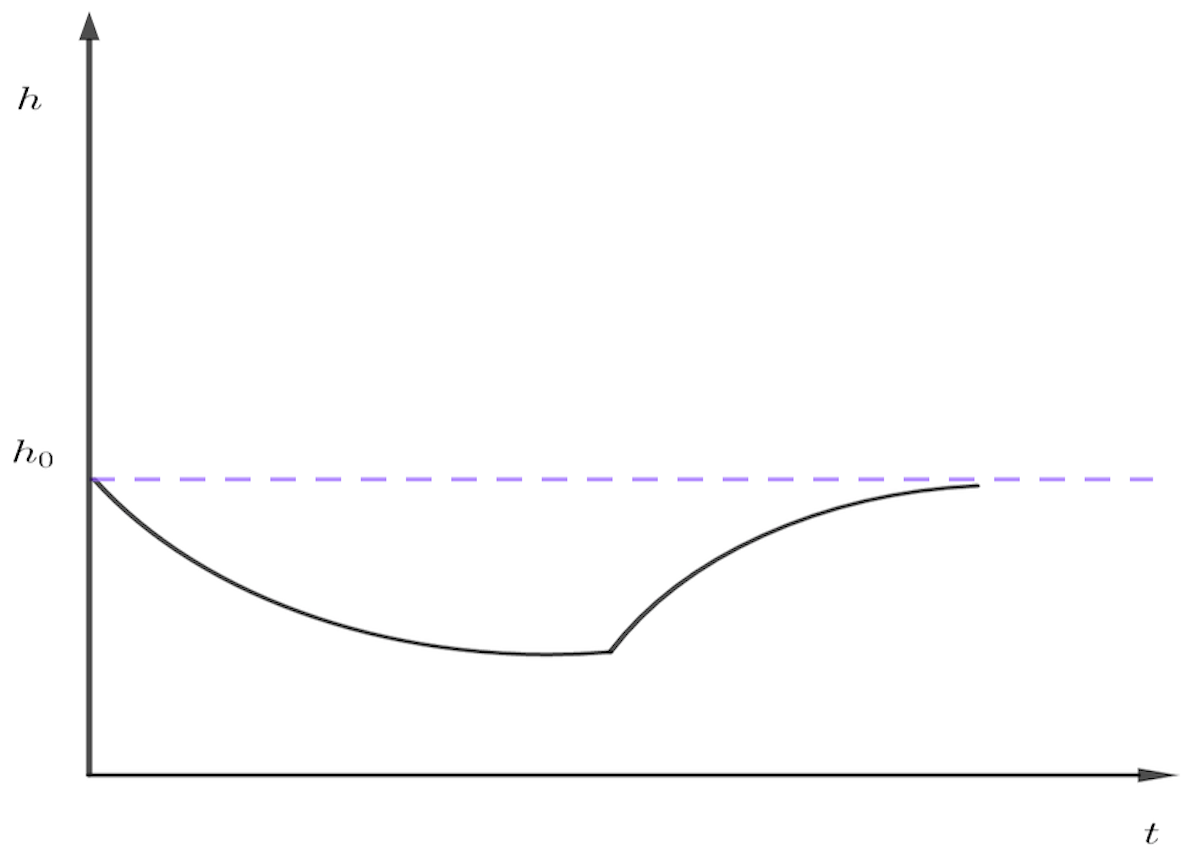
\includegraphics[width=\linewidth]{./img/pump_test1}
\end{figure}
\end{minipage}%
\begin{minipage}[t]{0.5\linewidth}
  \begin{figure}[H]
  \centering
  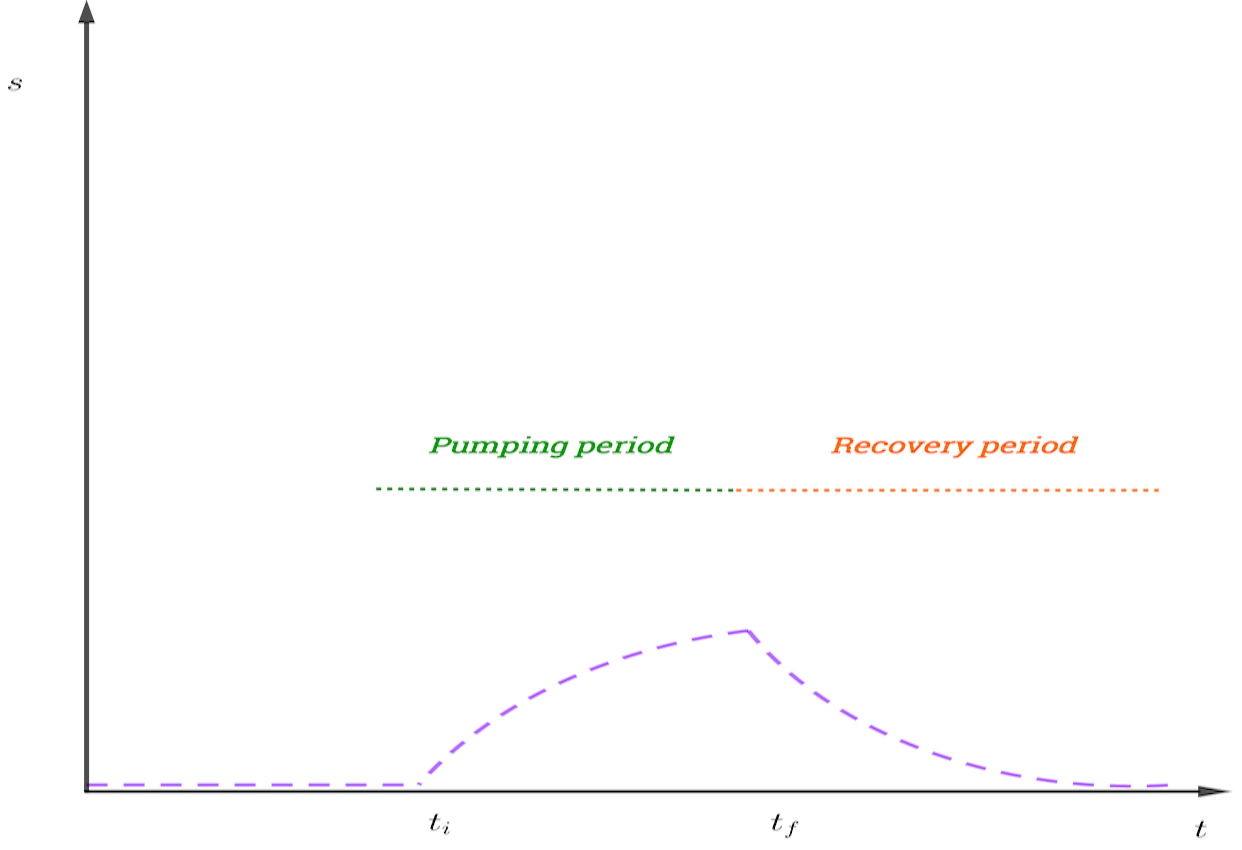
\includegraphics[width=\linewidth]{./img/pump_test2}
\end{figure}
\end{minipage}

And we have the following relations \footnote{ if $S\approx 0,2-0,4 \rightarrow$ free aquifer, if $S\approx 10^{-4}-10^{-3} \rightarrow$ confined aquifer}
\begin{equation*}
  \begin{cases}
     m =\der{\log(t)}s = 0.183\frac{Q}{T}\\
     S = \frac{2,25 T t_i}{r^2}
  \end{cases}
\end{equation*}

\section{Well hydraulics} % (fold)
\label{sec:well_hydraulics}
\subsection{Superposition theory} % (fold)
\label{sub:superposition_theory}
The contribution of n wells \footnote{Only the wells where $ |(x_0,y_0) - (x,y)|<R|$} at $t=t_0$
\[
  s((x_0,y_0),t_0) = \sumin s_i((x_0,y_0),t_0)
\]
\underline{Steady}
$$s(x_0,y_0) = \sumin \frac{Q_i}{2\pi T}\ln \left(\frac{R}{r_i}\right)$$
\underline{Transitory}
\[
  s((x_0,y_0),t) = \sumin \frac{Q_i}{4\pi T}\ln \left[\frac{2,25 T}{r_i^2s}(t-t_i)\right]
\]

% subsubsection transient (end)
% subsubsection steady_state (end)
% subsection superposition_theory (end)
\subsection{Boundaries} % (fold)
\label{sub:boundaries}
\subsubsection{Impervious boundary} % (fold)
\label{ssub:impervious_boundary}
\underline{Steady}
\[
  s(x_0,y_0) =  \frac{Q}{2\pi T}\ln \left(\frac{R^2}{r r^{\prime}}\right)
\]
\underline{Transitory}
\[
  s((x_0,y_0),t) =  \frac{Q}{2\pi T}\ln \left[\frac{2,25 T}{r r^{\prime}s}(t-t_i)\right]
\]
% subsubsection impervious_boundary (end)
\subsubsection{Fixed head boundary} % (fold)
\label{ssub:fixed_head_boundary}
\underline{Steady}
\[
  s(x_0,y_0) =  \frac{Q}{2\pi T}\ln \left(\frac{r^{\prime}}{r}\right)
\]
\underline{Transitory}
\[
  s((x_0,y_0),t) = s(x_0,y_0)  =  \frac{Q}{2\pi T}\ln \left(\frac{r^{\prime}}{r}\right)
\]
% subsubsection fixed_head_boundary (end)
\begin{figure}[H]
  \centering
  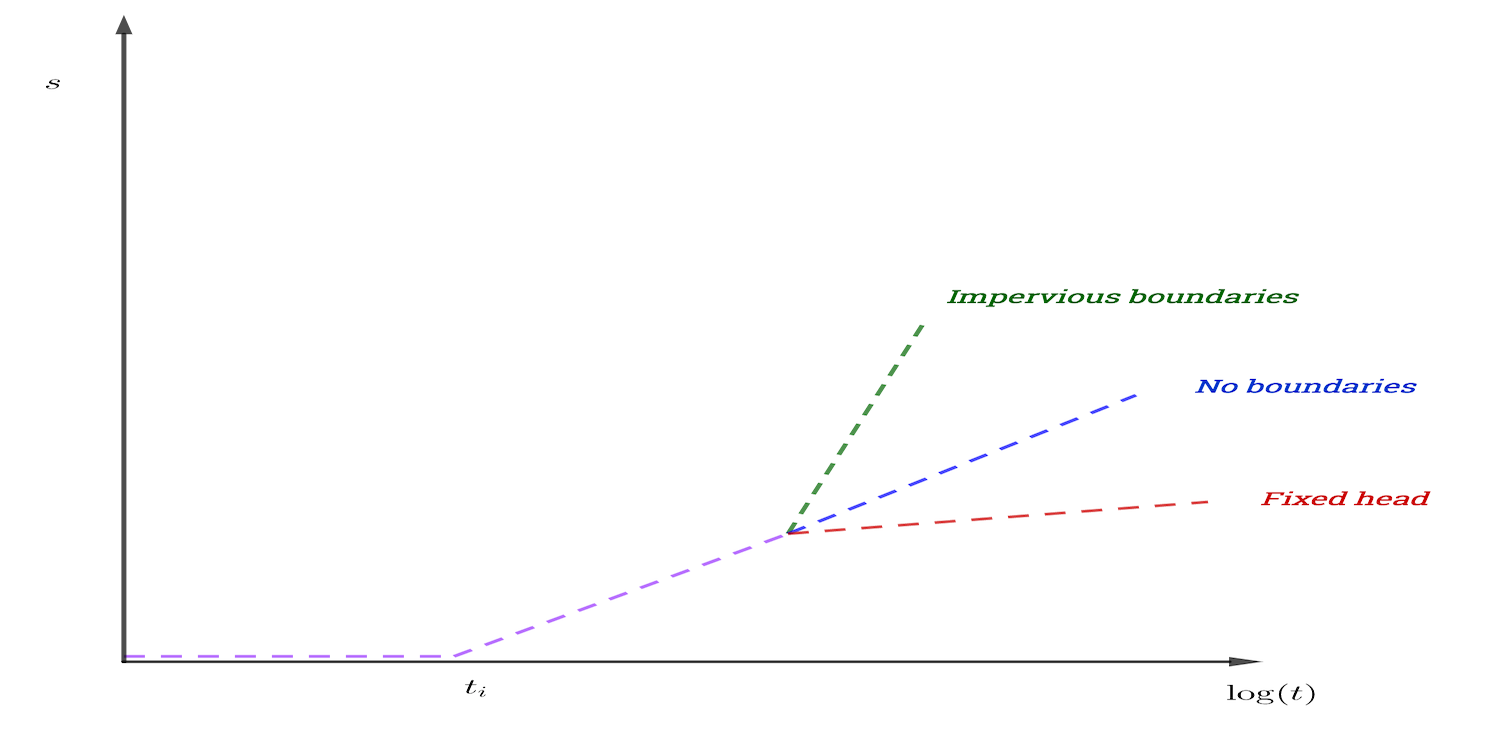
\includegraphics[width = 0.8\linewidth]{./img/pump_test3}
\end{figure}

\section{Pollution} % (fold)
\label{sec:pollution}
\subsection{Advection} % (fold)
\label{sub:advection}
  \begin{gather}\label{eq:2.1}
      \begin{cases}
         v= \frac{q}{\phi} = -\frac{K}{\phi} \pder{x}h\\
         F = v\phi C\\
         \pder{t}C= - v\pder{x} C
       \end{cases} \notag\\
      \shortintertext{where}
      \begin{aligned}
        & v: \emph{ is the average velocity in the flow direction}
      \end{aligned}\notag
  \end{gather} 
  \begin{gather}\label{eq:2.1}
      \begin{cases}
         \pder{t}C = D\cdot \Delta C & \emph{ difusion + dispersion eq} \\
         \pder{t}C = D\cdot \Delta C -v\pder{x}C& \emph{ advection eq}
       \end{cases} \notag\\
      \shortintertext{where}
      \begin{aligned}
        & D: \emph{ is the difusivity vector}
      \end{aligned}\notag
  \end{gather}
  \begin{gather}\label{eq:2.1}
      \begin{cases}
         C_{max} = \frac{M}{\phi b 4\pi t \sqrt{D_L D_T}} \\
         C = \frac{M}{\phi b 4\pi t \sqrt{D_L D_T}} \exp \left[ \frac{-(x-vt)^2}{4D_L t} -\frac{-y^2}{4D_T t} \right]
       \end{cases} \notag\\
      \shortintertext{where}
      \begin{aligned}
        & M = \frac{C_0 V_0}{M_{molar}}
      \end{aligned}\notag
  \end{gather} 
\subsection{Hydrodinamic dispersion} % (fold)
\label{sub:hydrodinamic_dispersion}
  \begin{enumerate}
    \item Molecular difusion (Fick’s laws)
    \item Mechanical dispersion
  \end{enumerate}
% subsection hydrodinamic_dispersion (end)Hydrodynamic dispersion
    \begin{gather}\label{eq:2.1}
      \begin{cases}
        F = -D_d\pder{x}C & \emph{ Fick’s first law}\\
        \pder{t}C = -D_d\pdder{x}C & \emph{ Fick’s second law}
       \end{cases}\notag \\
      \shortintertext{where}
      \begin{aligned}
        & F: \emph{ is the amount of solute per unit area} \\
        & D_d: \emph{ is the diffusivity}\\
        & C: \emph{ is the solute concentratios}\\
      \end{aligned}\notag
      \end{gather}

    \begin{gather}\label{eq:2.1}
      \begin{cases}
         D_L = \alpha_Lv_L+ D_d\\
         D_T = \alpha_Tv_T+ D_d
       \end{cases} \notag\\
      \shortintertext{where}
      \begin{aligned}
        & \alpha_L: \emph{ is the dispersivity} \\
        & L, \ D: \emph{account for longitudinal and transversal}
      \end{aligned}\notag
      \end{gather}

    \begin{table}[H]
      \centering
      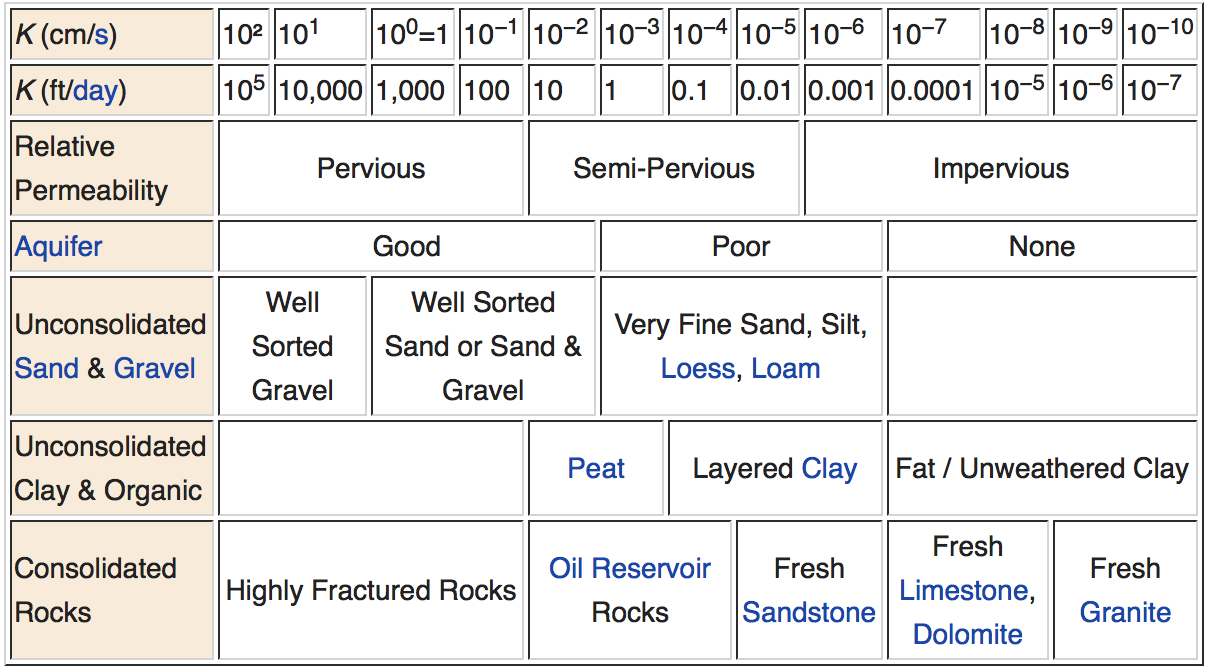
\includegraphics[width =.9\linewidth]{./img/table}
    \end{table}
    \textbf{Conversion}:
    \begin{align*}
        1ft = 0,3048 m \qquad \qquad \frac{1}{86,4}\frac{m^3}{day} = \frac{L}{s}
    \end{align*}
% section pollution (end)
% subsection boundaries (end)

% section well_hydraulics (end)

\newpage

\addcontentsline{toc}{section}{References}
\nocite{*}
\printbibliography
\end{multicols*}

\end{document}
